\chapter{Theoretical aspects}

\section {State of the art}

\tab During the development process of a software system new classes and new methods to the existing classes are added in order to fulfill new functionalities. All of the adding actions from above have a direct impact on the system structural dependencies. Those are the result of the source code analysis of the system. \\The source code is any static, textual, human readable, fully executable description of a computer program that can be compiled automatically into an executable form \cite{ct1}.\\On the other hand logical dependencies also can be added during the development process. Logical dependencies refer to those depencencies between entities that are not always visible through source code analysis. Logical dependencies can be easily extracted from the versioning system (e.g. Subversion , Git) commits.  (Figure \ref{fig:fig1}).

\tab The ideal situation presumes that changes in one part can be made without changing parts that are in a dependency relation with that part. Those dependencies affect the maintainability of the system and increase the realization effort of any problem that appears during the maintenance time. Studying only the structural dependencies of the system is not enough to get a clear overview of the system dependencies. For more precise results is needed a study that combines structural dependencies and logical dependencies. \\ We have analysed 19 open-source software systems of different sizes to investigate the links between structural dependencies and logical dependencies. 


\begin{figure}[h]
\centering
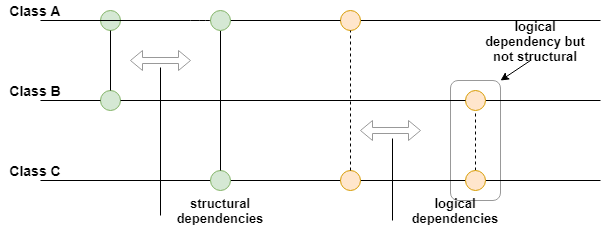
\includegraphics[scale=0.60]{fig1.png}
\caption{Relationships between structural and logical dependencies }
\label{fig:fig1}
\centering
\end{figure}

\section{Software dependencies}
\tab A dependency is created by two elements that are in a relationship and indicates that an element of the relationship, in some manner, depends on the other element of the relationship. In this case, if one of these elements change, there could be an impact to the other \cite{ct2}. Dependencies are discovered by analysis of source code or from an intermediate representation such as abstract syntax trees \cite{ct3} .

\section{Structural dependencies}
\tab Structural dependencies (a.k.a syntactic dependencies or structural coupling) are the result of source code analysis. Each source code file can contain one or more classes \cite{ct4}.\\

In object-oriented programming, a class is an template for creating objects that provides initial values for member variables and implementations of functions or methods. \cite{oopconcept}\\
\tab In the following we will present the class components and how those components can introduce software dependencies with other classes.

Class components to discuss :
\begin{itemize}
  \item Class name. Inheritance.
  \item Comments.
  \item Attributes. 
   \item Constructors.
   \item Methods.
\end{itemize}


\subsubsection{Class name. Inheritance}
The user-defined objects are created using the class keyword. The class is a blueprint that defines a nature of a future object. 
The name of the class is the name located after the keyword class. During the structural analysis of the projects the classes names are extracted in order to identify the structural dependencies elements names .

\begin{lstlisting}[language=java, caption={Class declaration.}]
public class A {
}
public class B extends A {
}
\end{lstlisting}

A structural dependency between a class and other class can be given by inheritance. Inheritance can be defined as the process where one class acquires the properties of another class \cite{oopconcept} .\\
The class which inherits the properties of other class is known as subclass and the class whose properties are inherited is known as superclass (a.k.a base class, parent class). The name of the superclass is the name located after the keyword extends .

\subsubsection{Comments}
Comments are statements that are not executed by the compiler and interpreter. The comments can be used to provide information about a variable, method or any other statement. There are multiple types of comments :\\

\textit{/* text */} -  ignores characters from begining of /* to */.\\
\textit{/** documentation */} -  indicates a documentation comment, just like comments that use /* and */.\\
\textit{// text} -  ignores everything from // to the end of the line.\\ 

Comments never introduce any kind of structural dependencies. They are used just for the source code intelligibility.

\subsubsection{Attributes}

Attributes represent the state of the object because they store the information about the object. An attribute is another term for a field. \\

\textit{private B b;}\\
The keyword private signifies that a method or variable can be accessed only within the declaring object. The keyword public allows access also from outside of the object \cite{oop2}, \cite{ct11} .

The attributes or members of a class can lead to structural dependencies between the class and the class types of the attributes.

\subsubsection{Constructors}

A constructor of a class is a member function that is executed whenever we create a new object of that class.  A parameterized constructor introduces new structural dependencies by its parameters.

\subsubsection{Methods}

Some of these attributes and methods are publicly visible from outside the object:  the interface. Other
attributes and methods are for private use of the object itself : the implementation. Either ways when studying structural dependencies the publicity of an attribute or of a method is irrelevant. \cite{oopconcept} The relevant part is the type of the attribute or the return type and the parameters of the method. A method can introduce structural dependencies in three ways : by its return type , by its call parameters or by its local variables .\\

\tab On the other hand, even though in some of the cases if class A depends on class B , changes in class B can produce changes in class A, but not the other way around \cite{ct5} . There are other cases in which if class A depends on class B, changes in class B can produce changes in class A and viceversa if we are speaking in the context of a new feature implementation that implies changing return types and adding new methods. So we will consider structural dependencies as bidirectional relationships, "classA depends on class B" and "class B depends on class A".\\ \tab The choice of building bidirectional relationships is motivated by the fact that we cannot establish for the moment the direction of the logical dependencies of the system. So in order to have a omogeninty between the logical and structural dependencies analysis results, we will take both of the relationships types as bidirectional. 

\section{Logical dependencies}
\subsection{Version control systems}
In computer software engineering, revision control is any kind of practice that tracks and provides control over changes to source code. Software developers sometimes use revision control software to maintain documentation and source code.\\
At a basic level, developers could retain multiple copies of the different versions of the program and label them appropriately. This method can work but it is inefficient as many copies of the program have to be maintained. Because of this, systems to automate some or all of the revision control process have been developed. 
\\ 
\tab Among the keywords used in a versioning system we can mention:\\
\textit{\textbf{Repository}} -  is a virtual storage of a project. It allows to save versions of the code, which can be access when needed.\\
\textit{\textbf{Master/Trunk}} - the main body of development, originating from the start of the project until the present.\\
\textit{\textbf{Branch} }- a copy of code derived from a certain point in the master that is used for applying major changes to the code while preserving the integrity of the code in the master. The changes are usually merged back into the master.\\
\textit{\textbf{Revision}} - changes are usually identified by a number or letter code, that code is known as "revision".\\


\subsection{Definition}

\tab  In software engineering, we use co-evolution to represent the phenomenon in software evolution that change in one component C2 in response to a change in another component C1 \cite{ct5}, \cite{ct6}, \cite{ct8}. 
There are differences between co-evolution and evolutionary coupling.\\
\tab Co-evolution is the result of cause–effect changes between two components: changes to one component require changes to another component. On the other hand, evolutionary coupling is based on the evolution history of two components and is a measurement of the observation that two components are changed at the same time.\\ 
\tab  Modifications made to two components at the same commit do not necessarily indicate the co-evolution of the two. These modifications could be completely unrelated.\\ So, evolutionary coupling could also be determend accidentally by two components changing in the same commit and it will bring noise to the measurement of evolutionary coupling.  \cite{ct5} \\ We will try to filter that noise by setting different thresholds in the process of analysing the systems.

\tab The versioning system contains the long-term change history of every file. Each project change made by an individual at certain point of time is contained into a commit \cite{ct7}.All the commits are stored in the versioning system cronologicaly and each commit has a parent. The parent commit is the baseline from which development began, the only exeption to this rule is the first commit which has no parent. We will take into consideration only \textit{commits that have a parent} since the first commit can include source code files that are already in development (migration from one versioning system to another) and this can introduce reduntant logical links \cite{ct8} .\\

\tab The number of files changed in a commit can influence the logical dependencies. A relatively big number of files changed can indicate a merge of all changes from another branch as a single commit or a folder renaming. This can lead to a number of logical dependencies that are redundant since the files are not actualy changing in the same time.The logical dependencies are splitted into three categories :\\ \\
\textit{\textbf{Category 1:} Dependencies found in commits with less than 5 source code files changed.}\\
\textit{\textbf{Category 2:} Dependencies found in commits with more than 5 files changed but less than 20. }\\
\textit{\textbf{Category 3:} Dependencies found in commits with more than 20 files.}\\

\tab Also, files that changed only by comments change can lead to redundant logical dependencies. If class A and class B change together but the only change was a change in the comments then there may not be any logical dependency between them. 
For each category mentioned above, two dependencies analysis will be made:
\textit{\textbf{A:} Considering comments  as valid changes.}
\textit{\textbf{B:} Considering comments  as redundant changes. }
In the second case if class A and class B change together but the only change found is a comment change then between class A and B will not be set a logical dependency.\\

\tab Another filtering method that can lead to a more accurate results is to count the occurrences of the logical dependencies. If class A and class B change together but only once during all the commits from the active branch the class A and B may or may not represent a logical dependency.
